\label{sec:tangle}

\begin{figure*}
    \centering
    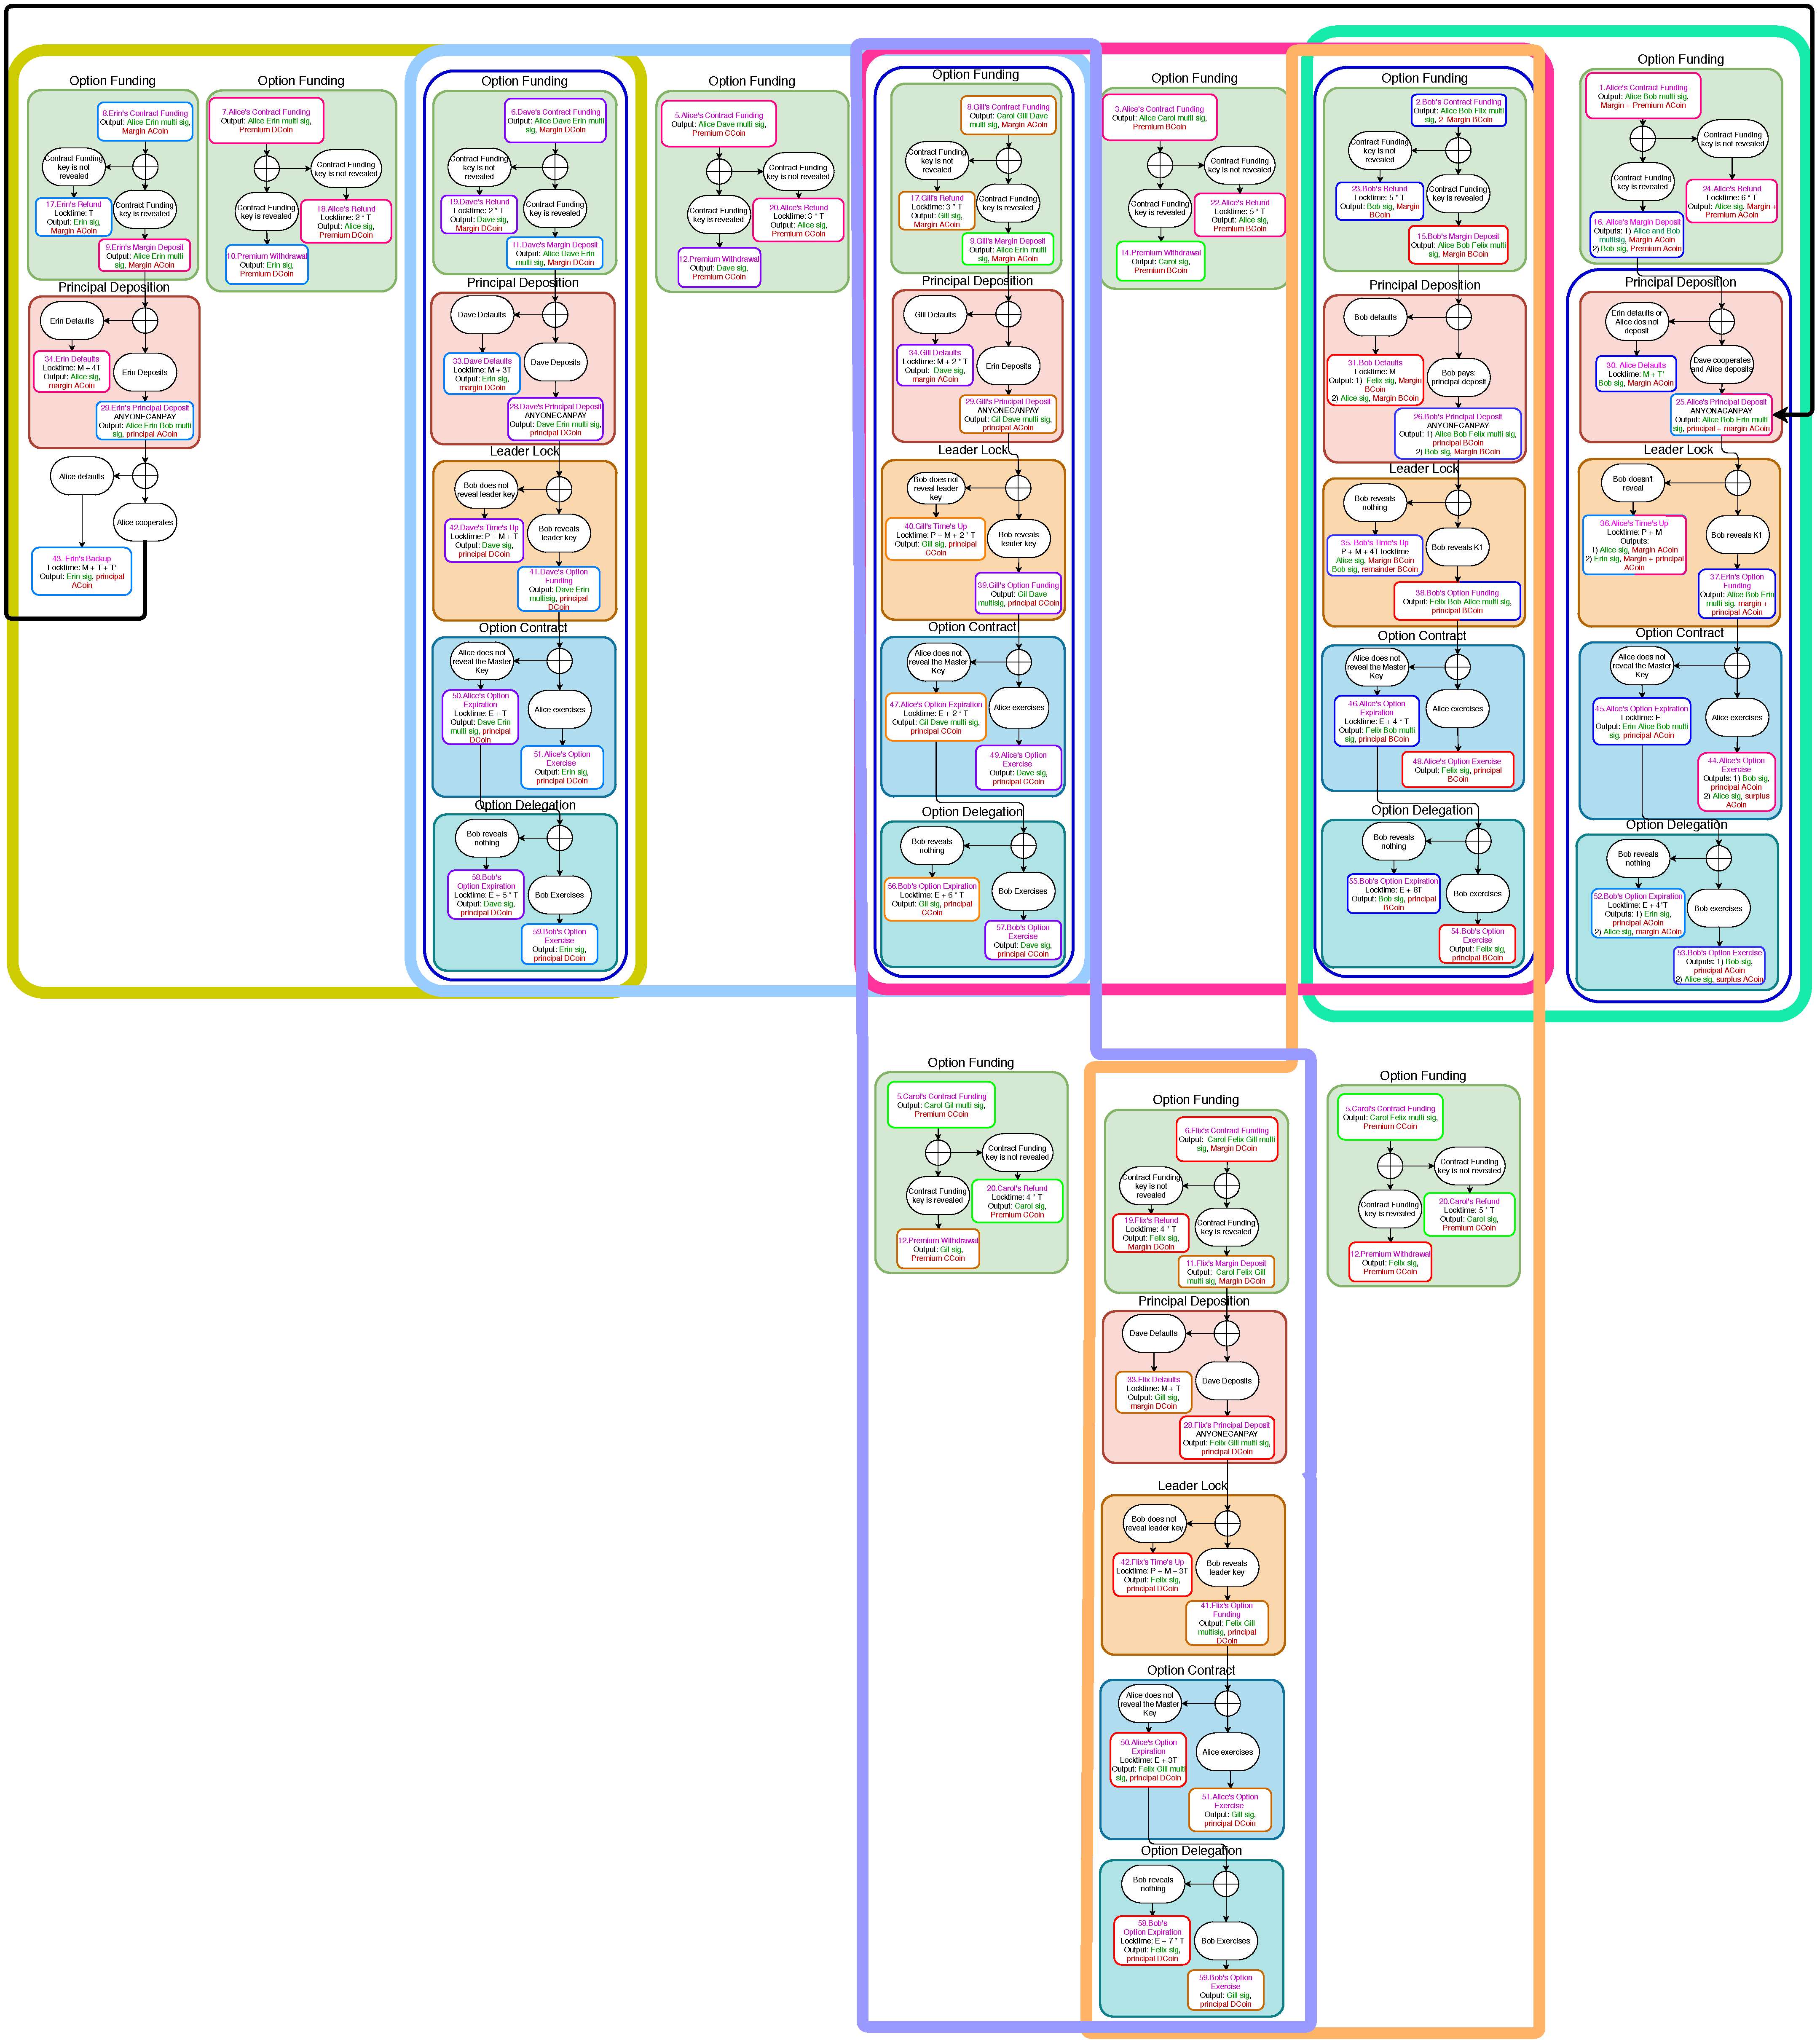
\includegraphics[
    width=\textwidth,
    ]{figures/tangle.pdf}
    \caption{a tangle of two arbitrage loops; one for Alice and one for Carol}
    \label{fig:tangel}
\end{figure*}

So far, we have studied an arbitrage with one exploiter and all other parties only as sellers. Now, imagine each of the sellers can be an exploiter in a second arbitrage using the principal from the first arbitrage. We call such intertwined arbitrages as tangled money market whose example is shown in Fig.~\ref{fig:tangel}. Furthermore, these tangled swaptions do not have to be in the form of arbitrage. In other words, a series of swaptions entangled together is counted as a tangled money market. In this section, we prove two theorems for tangles. And by designing a protocol we provide a constructive proof for our final theorem.

Note each transaction may have multiple inputs and outputs in real word. We only consider those transaction involved in a tangle have single input and output. 
% inputs and outputs whose both source and destination transactions are involved in the tangle.
We define $P=\{p_1,\ ,p_2,\ ..,\ p_n\}$ as the set of distinct parties which are participating in the tangle even through different accounts.

First of all, to analyse a tangle we introduce two graph models:

\begin{enumerate}
    \item Swaptions graph: $\mathcal{G}_s=(V, E)$ where $V$ is the finite set of vertices each representing a swaption, and $E$ the finite set of edges. Each edge is an ordered pair of vertices. In a set of overlapping swaptions, each swaption is shared between three parties $p_1, p_2, p_3$, where $p_1$ is the buyer of the swaption. In order to build the $\mathcal{G}_s$, each of these swaptions is shown as two separate swaptions; one between $p_1$ and $p_2$, and the other one between $p_1$ and $p_3$. This is another interpretation of the overlapping process. Where in real world, $p_1$ is an intermediary who mediates between $p_2$ and $p_3$, in this interpretation, she actually takes $p_2$'s principal to deposit in the swaption between herself and $p_3$. For each vertex $v \in V$ there are two functions $\beta: V \to P$ and $\sigma: V \to P$ which indicate the swaption buyer and seller respectively. Each edge represents transfer of principal between two swaptions. An example of this graph is shown in Fig.~\ref{fig:gen-graph}.

    
    \item Principal flow graph: This graph represents the flow of principal and \keyone key. $\mathcal{G}_{p} = (V_p,E_p)$ where $V_p$ is the finite set of vertices and $E_p$ the finite set of edges.
    For each swaption in $\mathcal{G}_s$ there are two vertices in $V_p$ corresponding to it. Each of them represents a party in the swaption. The function $\ell(v)$ where $\ell(v): V_p \to P$ returns the party related to vertex $v$. Each $e \in E_p$ is an ordered pair of vertices $(h(e), \tau(e))$ that $h(e)$ and $\tau(e) \in V_p$. For the above example there would be four vertices with labels $p_1, p_2, p_1$ and $p_3$. Clearly, there is a correspondence between each vertex of $\mathcal{G}_s$ to a pair of vertices in $\mathcal{G}_{p}$. We define the function $\rho: E_p \to \{i, x, t\}$, such that the following properties hold:
    \begin{itemize}
        \item For each $e \in E_p$ that $\rho(e) = i$, $e$ connects two vertices of one swaption and represents the deposition order inside a swaption \ie $h(e)$ has to deposit earlier than $\tau(e)$ by the locktime rules. Note that for each $v \in V_p$, there is a unique $e \in E_p$ such that $v$ is either $h(e)$ or $\tau(e)$, since each vertex is participating in a single swaption. We define function $\mathcal{O}: V_p \to V_p$ where for a vertex $v, \mathcal{O}(v)$ is the other vertex connected to the unique edge $\Tilde{e}$ with $\rho(\Tilde{e}) = i$ connected to $v$.
        
        \item For each $e \in E_p$ that $\rho(e)=x$, $e$ represents the flow of principal between swaptions i.e. the principal moves from $h(e)$ to $\tau(e)$. We also define successor and precursor of a vertex as the functions $s: V_p \to V_p  \cup \O $ and $p: V_p \to V_p \cup \O$ such that for each $v \in V_p$ if there is $e \in E_p$ that $\rho(e)=x$ and $h(e)=\mathcal{O}(v)$ then $s(v)=\tau(e)$ and if there is no such $e$ then $s(v)=\O$ and for each $v, u \in V_p$ if $s(v)$ is $u$ than $p(u)$ is $v$ and if there  is no $v \in V_p$ such that $s(v)$ is $u$, then $p(u)$ is $\O$. Functions $s$ and $p$ are well-defined since there can not be any two edges $v$ and $u$ with $\rho(v) = \rho(u)= x$ such that $h(u) = h(v)$ or $\tau(u) = \tau(v)$. As an intuition, given our previous example, the successor of $p_1$'s vertex corresponding to the swaption with $p_2$ is his vertex corresponding to the swaption with $p_3$, and the precurser of $p_1$'s vertex corresponding to his swaption with $p_3$ is his vertex correspondingo the swaption with $p_2$.
        
        The $\mathcal{G}_{p}$ graph of previous example is shown in Fig.~\ref{fig:prin-flow-graph}. It is clear that for each $v \in V_p$, $\ell(s(v)) = \ell(v)$, since otherwise the party $\ell(v)$ transfers his asset to party $\ell(s(v))$ without getting anything back, which is not rational. With the same argument, $\ell(p(v))$ is equal to $\ell(v)$. We call this, the rationality property of $\mathcal{G}_{p}$.
        
        \item Consider all $v \in V_p$ that there is no edge $e \in E_p$ that $\rho(e) = x$ and $\tau(e) = v$. Then, for each $i \in \mathbb{N}$ that $\mathcal{O}(s^i(v)) \neq \O$, there is an edge $e'$ that $\rho(e') = t$ and $\tau(e') = v$ and $h(e') = \mathcal{O}(s^i(v))$. This type of edge, will later be used to impose a deposition order between two vertices in two adjacent swaptions in order to guarantee the safety of parties who inject principals to the system rather than transform it from another swaption.
        
        % \ahC{Definition has to be if and only if, but I don't know how}
        
        % if $\rho(e)=t$, then there is an $i \in \mathbb{N}$ that $h(e) = \mathcal{O}(s^{i}(\tau(e)))$ and there is no $b \in E$ that $\rho(b)=x$ and $\tau(b)=\tau(e)$.
        % \melikaC{I don't understand! yani in poolaro bayad az jib avorde bashe, na in ke ba ye edge e x i avorde bashe}
    \end{itemize}
    % See Fig.~\ref{fig:prin-flow-graph}.

It is worth mentioning that in $\mathcal{G}_{p}$ there is no cycle $c$ that for all of its edges $e$  $\rho(e) = x$, since otherwise the principal transferred through $c$ would not have any sources.

\end{enumerate}



\begin{figure}
    \centering
    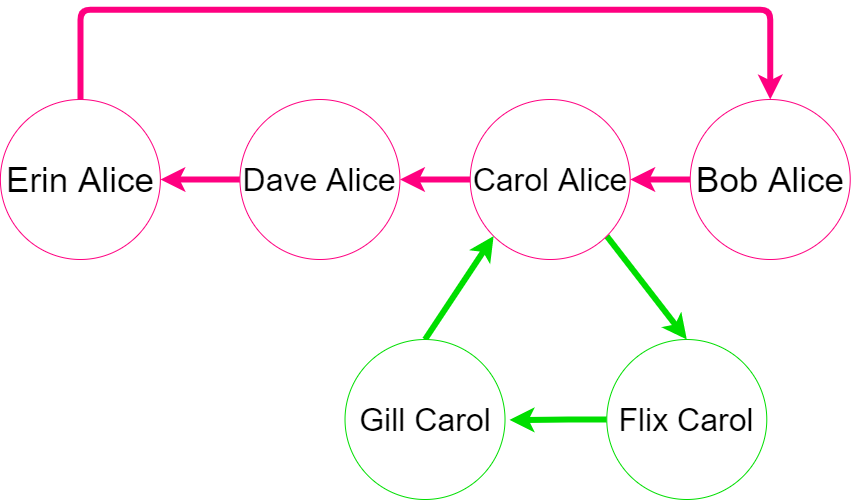
\includegraphics[width=0.7\textwidth]{figures/gen-graph.png}
    \caption{Example for \genGraph graph}
    \label{fig:gen-graph}
\end{figure}

\begin{figure}
    \centering
    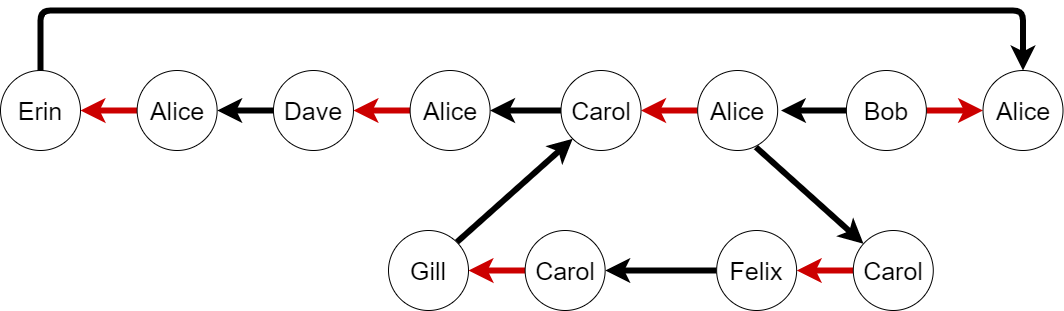
\includegraphics[width=\textwidth]{figures/prin-flow-graph.png}
    \caption{Example for $\mathcal{G}_{p}$ graph}
    \label{fig:prin-flow-graph}
\end{figure}

% \begin{figure}
%     \centering
%     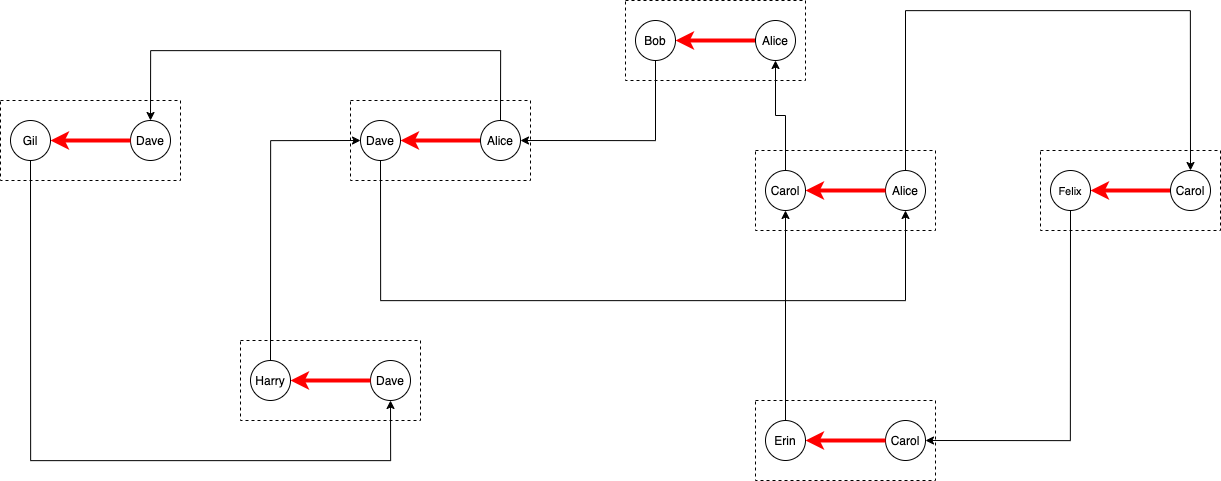
\includegraphics[width=\textwidth]{figures/lock-imposition-graph.png}
%     \caption{Example for \AtwoGraph Graph}
%     \label{fig:lock-impos-graph}
% \end{figure}


\begin{definition}{\it Concurrent Tangle}\\
A tangle $T$ is concurrent if the \genGraph graph representing $T$ is a \scdg.
\end{definition}


\begin{definition}{ Association Set}\\
In the $\mathcal{G}_s$ graph, a vertex $v$ is in the association set of party $p_i$ if $\beta(v) = p_i$ or $\sigma(v) = p_i$.

\end{definition}

For later usage, we need to find the $p_{master}$ for a tangle.
Given a \genGraph graph $\mathcal{G}_s=(V, E)$ of a tangle $T$, we design a graph $\mathcal{G}_{r}=(V_r,E_r)$ such that $V_r=\mathcal{P}$ and for every $v \in V$ there is an edge $\hat{e} \in E_r$ for which $h(\hat{e}) = \beta(v)$ and $\tau(\hat{e}) = \sigma(v)$. Each vertex of $\mathcal{G}_{r}$ from which all the vertices are reachable \cite{bang2008digraphs} is a candidate whose label is eligible to be the $p_{master}$ of $T$.
% Note that strongly connected property of swaptions graph of $T$ is neccessary (not enough) condition to find an eligible $p_{master}$ for $T$. Therefore, if 
% \begin{algorithmm}
% {\it Owner Finder}
% \label{algo:owner-finder}
% \\
% \end{algorithmm}
% \begin{algorithm}
% \caption{Master finder}
% \begin{algorithmic}
% \State $\mathcal{C}=\mathcal{P}$
% \For{$i$ \textbf{from} $0$ \textbf{to} $n$}
%     \For{$j$ \textbf{from} $0$ \textbf{to} $n$}
%         \If {there is no path from $v_i$ to $v_j$ in $\mathcal{G}_{t}$}
%             \State remove $p_i$ from $\mathcal{C}$
%             \State break
%         \EndIf
%       \EndFor
%     % \State add $p_i$ to $\mathcal{C}$
%  \EndFor
%  \State return $\mathcal{C}$
% \end{algorithmic}
% \end{algorithm}



% The output of the algorithm is the list of candidate labels which are eligible to be the $p_{master}$ of $T$. 

% A tangle $T$ is \AtwoOk if the algorithm~\ref{algo:owner-finder} outputs at least one candidate party. 

For every graph $\mathcal{G}_1=(V_1, E_1)$, according to the definition of {\it feedback edge set} previously stated in \cite{bondy2000graph}, given $L$ the feedback edge set of $\mathcal{G}_1$ that $L \subseteq E_1$, the edge-induced subgraph $\mathcal{G}_2=(V_2, E_2)$ of $\mathcal{G}_1$ that $V_2=V_1$ and $E_2=E_1-L$ is acyclic.

\begin{definition}{\it Protected}\\
\label{def:pfok}
Assume subgraph $\mathcal{G}_{t}=(V', E')$ of $\mathcal{G}_{p}$ where $V'=V_p$ and $E'=\{e \in E_p | \rho(e) \neq t\}$.
A tangle $T$ is \keyoneOk if
\begin{enumerate}
    % \item $\mathcal{G}_{t}$ has only one source. We call this source, the \depsrc of $T$ and assume $\ell(\depsrc) = p_{leader}$.
    \item For all the source\footnote{A vertex $v$ in the graph such that there is no edge $e$ that $\tau(e) = v$} vertices $v$ in $\mathcal{G}_{t}$, $\ell(v)$ has to be identical and we assume $\ell(v)=p_{leader}$.
    \item $\mathcal{G}_{p}$ has a feedback edge set $L=\{e_0, e_1, ..e_l\}$ that for all $e_i \in L$, $\ell(\tau(e_i))= p_{leader}$ and $\rho(e_i) \in \{i, t\}$. 
\end{enumerate}

\end{definition}

 
% As it is clear, if the tangle is \keyoneGraph acceptable, then its $\mathcal{G}_{pf}$ graph has no more than one source. Since the $\mathcal{G}_{pf}$ graph has more edges than its $SG$ subgraph. \fatemeC{maybe should move it}

% \ahC{How can we explain the exceptional cases in which two keyone holder randomly choose the same key, or by cooperating?}


\begin{definition}{\it Cooperable}\\
A concurrent tangle $T$ is cooperable if it is \keyoneOk and there is at least one party eligible to be its $p_{master}$.
% algorithm~\ref{algo:owner-finder} outputs at least one candidate party when executes on $T$.
\end{definition}


% For each concurrent tangle, we call the output party of algorithm~\ref{algo:owner-finder}, the \Atwo key holder of $T$.

Now, we provide an example for a cooperable tangle. Fig.~\ref{fig:example-swp} shows the \genGraph graph, and Fig.~\ref{fig:example-pf} represents the principal flow graph of this example. All the source vertices in the principal flow graph have the label $B$, thus the party $B$ is $p_{leader}$. The principal flow graph has a feedback edge set with all the edges pointing to $B$'s vertices. Additionally, the Fig.~\ref{fig:example-gr} shows the $\mathcal{G}_{r}$ in which there is a path from vertex $A$ to every other vertex. Therefore, the party $A$ is the $p_{master}$ of this concurrent tangle.
% the property mentioned in protected definition.  
% Fig.~\ref{fig:example-pf} shows the principal flow graph of a cooperable tangle.

\begin{figure}
    \centering
    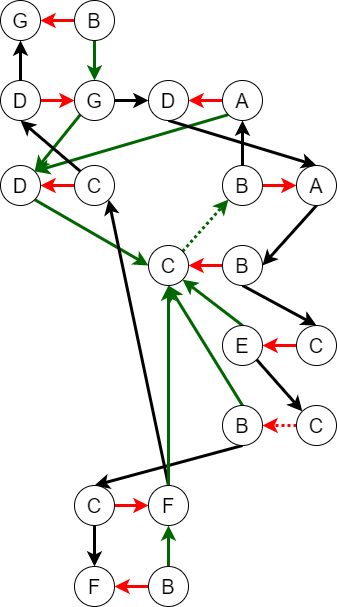
\includegraphics[width=0.8\textwidth]{figures/example.png}
    \caption{Principal flow graph of a cooperable tangle. Green, red and black edges represent edges whose $\rho$ function is equal to $t, x$ and $i$ respectively. Dotted edges are the feedback edge set of the graph.}
    \label{fig:example-pf}
\end{figure}
\begin{figure}
    \centering
    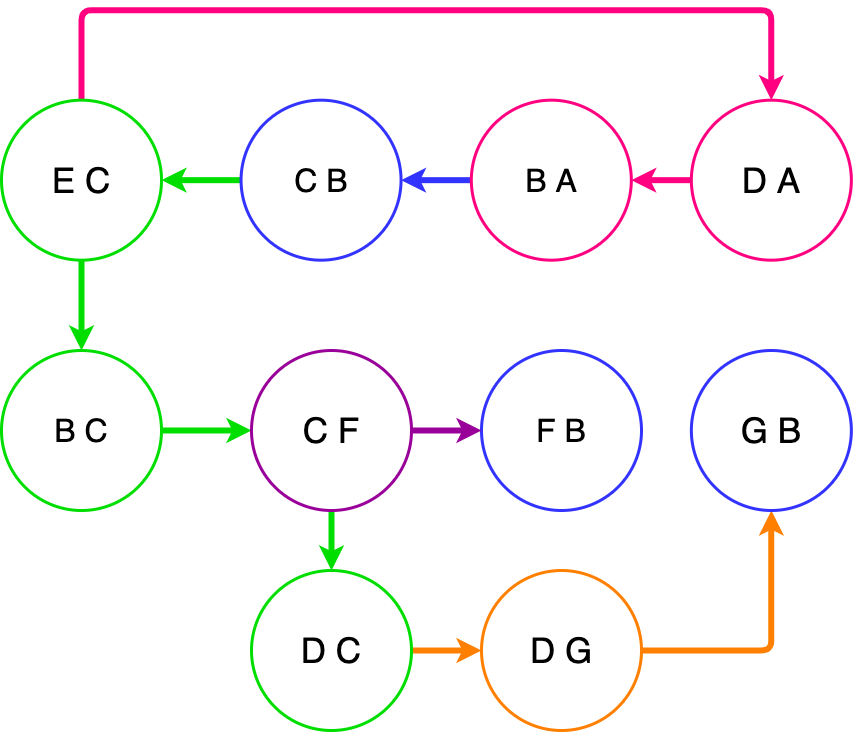
\includegraphics[width=0.5\textwidth]{figures/cooperable-example-swaption.png}
    \caption{Swaptions graph of a cooperable tangle. A node with the colors pink, blue, green, purple, and orange represents a swaption whose buyer is A, B, C, F, and G, respectively. The color of each edge represents the party who is transmitting the principal.}
    \label{fig:example-swp}
\end{figure}
\begin{figure}
    \centering
    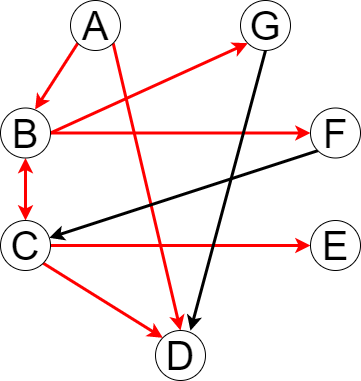
\includegraphics[width=0.5\textwidth]{figures/cooperable-example-tour.png}
    \caption{The $\mathcal{G}_{r}$ graph for our example to find the party $p_{master}$. Red edges show that the parties $B, C, D, E, F, $ and $G$ are reachable from party $A$.
}
    \label{fig:example-gr}
\end{figure}
Before delving into the first theorem, we need to define the required security property for executing such a tangle. To do so, we define multiple classes for the future of every distinct parties in the tangle. We assume that for a fix desired party, every other party can act cooperatively for cheating on him.

% \begin{figure}
%     \centering
%     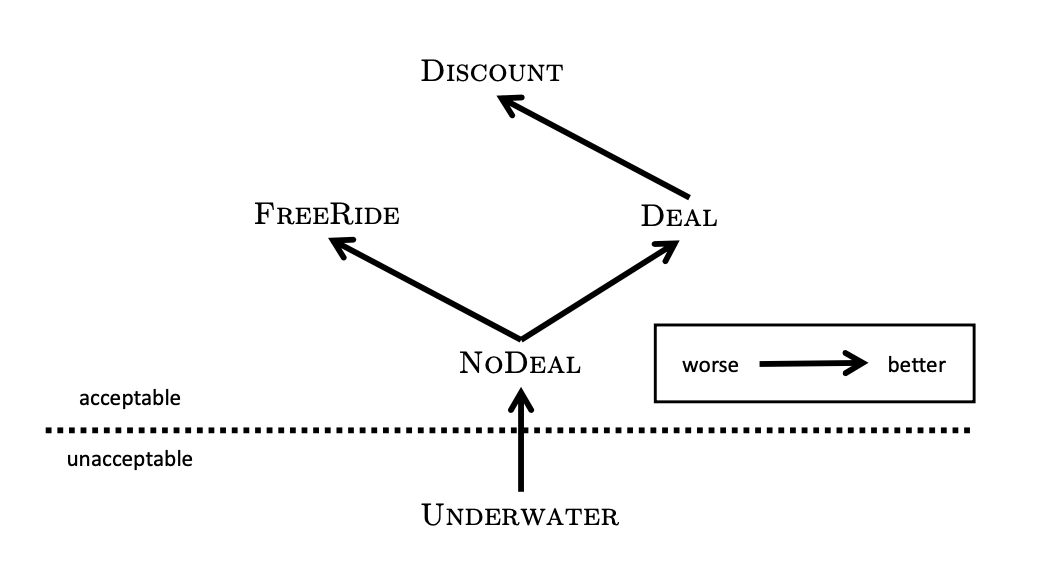
\includegraphics[width=\textwidth]{figures/outcomes.png}
%     \caption{The priority of feasible state in the point of view of each parties.}
%     \label{fig:outcomes}
% \end{figure}

To be consistent with prior terminology first introduced by Herlihy in his paper ``Atomic Cross-Chain Swaps", for a party $p_i$ we define these states \cite{herlihy2018atomic}:

\begin{itemize}
    \item Nodeal: There is no swaption in $p_i$'s {\it associated set}, that has been executed. Hence, he keeps his prior assets without getting any new assets.

    \item Deal: The swaptions in $p_i$'s association set are all properly executed and the amount of principals inside them are finally swapped.

    % \ahC{\item Discount: In at least one of swaptions in $p_i$'s association set, $p_i$ does not pay his principal while acquires other party's principal or premium and in all its other swaptions the principals are swapped completely.}

    \item Freeride: The party $p_i$ does not pay anything through the entire tangle while getting some asset as premium or principal at the end of execution phase.

    \item Underwater: In at least one swaption, he does not gain any new principal, while he loses his principal.

\end{itemize}
Now we can properly give a definition of the needed security property for our tangle: 
A protocol $P$ for a tangle $T$ is secure if after execution of $P$ on $T$, none of the parties who have adhered to $P$ enter the underwater state.
Next, it is time to state the first theorem:
\begin{theorem}
\label{th:concurrency}
For every cooperable tangle $T$, there is a secure protocol $P$.

\end{theorem}
% \begin{figure}[htp]

%     \caption{The conceivable shapes of a sink node. The blue dashed-line arc is optional.}
%     \subfloat[Form 1]{
%     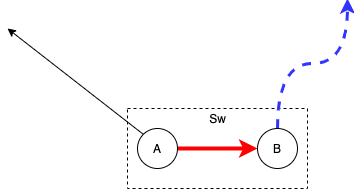
\includegraphics[width=0.45\textwidth]{figures/sink-node-2.png}
%     \label{fig:sink-1}
%   }~
%   \subfloat[Form 2]{
%   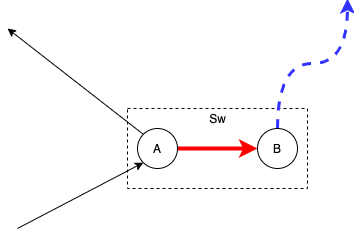
\includegraphics[width=0.45\textwidth]{figures/sink-node-4.png}
%   \label{fig:sink-2}
%   }
%   \label{fig:sink-shapes}
% \end{figure}
% \begin{figure}
%     \centering
%     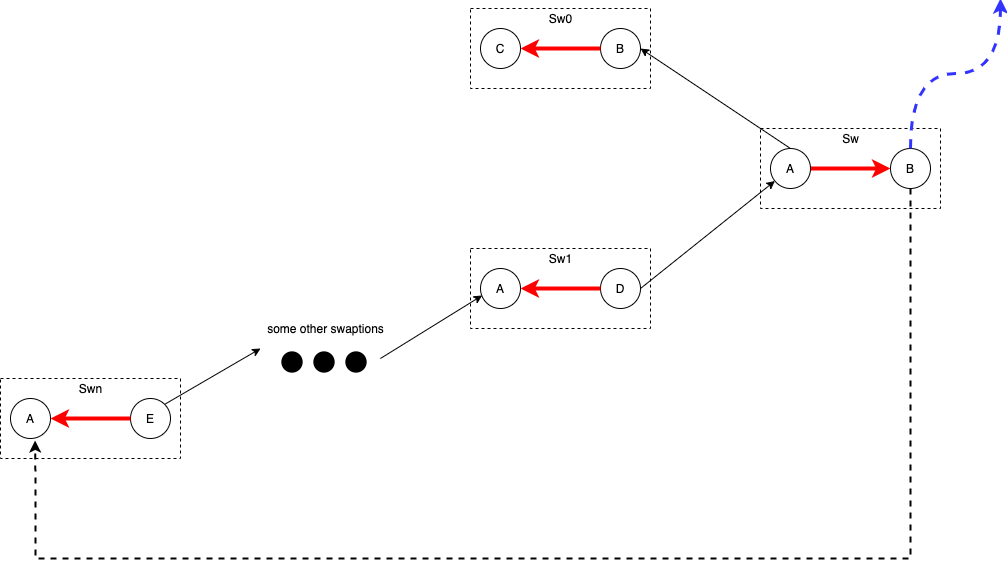
\includegraphics[width=\textwidth]{figures/sink-node-1.png}
%     \caption{The sink node which is the end of a line.}
%     \label{fig:sink-3}
% \end{figure}
% \begin{figure}
%     \centering
%     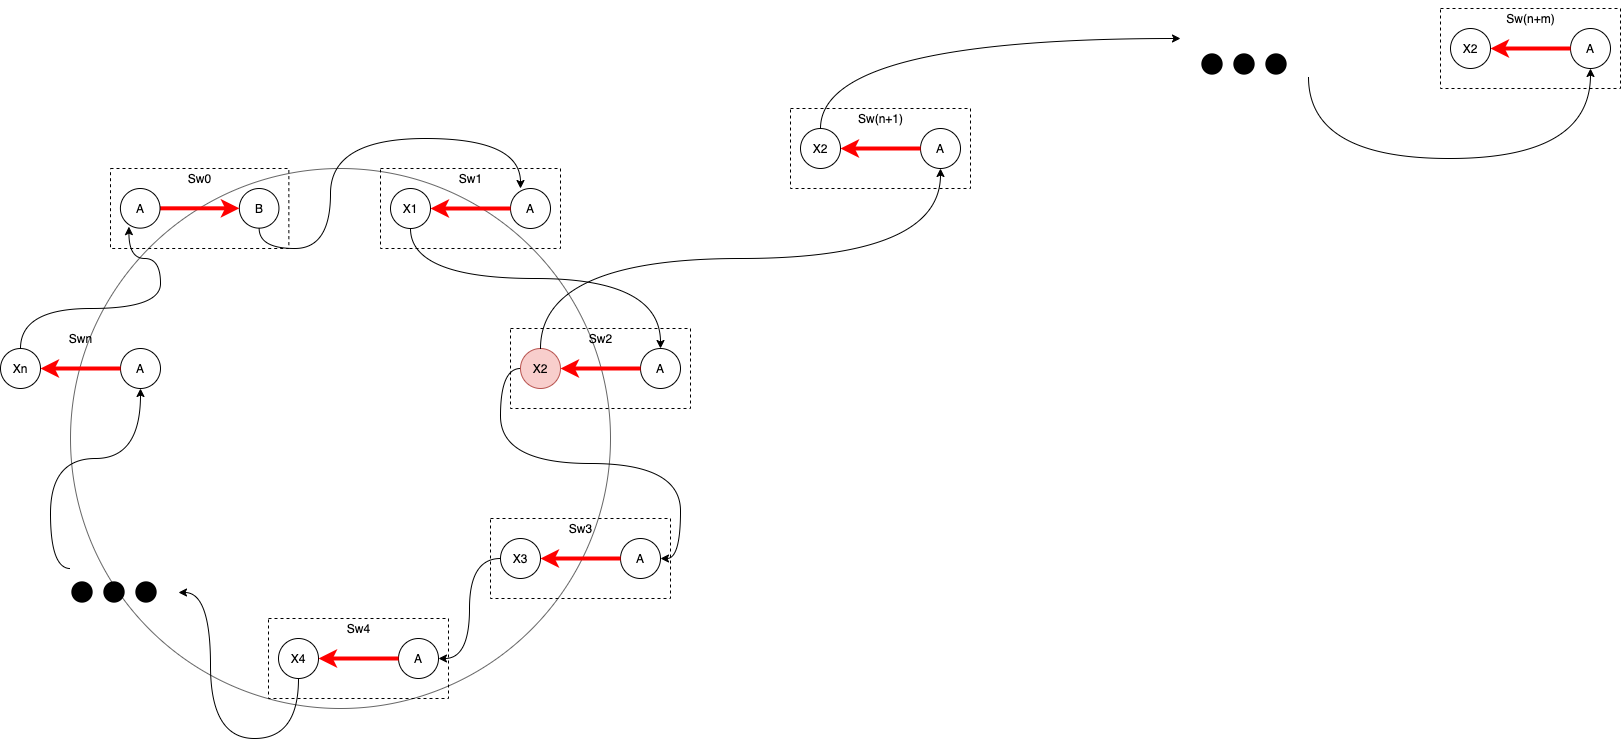
\includegraphics[width=\textwidth]{figures/sink-node-3.png}
%     \caption{The looped sink node.}
%     \label{fig:sink-4}
% \end{figure}
\begin{lemma}
\label{lm:sink}
In the edge-induced subgraph $\mathcal{G}_k=(V_k, E_k)$ of $\mathcal{G}_{p}=(V_p, E_p)$ of the concurrent \keyoneOk tangle $T$, that $V_k = V_p$ and 
% edges $e \in E$ that $\tau(e) = p_{leader}$ and $\rho(e) \in \{i, t\}$ are removed in $E'$,
$E_k = E_p - \{e \in E_p \ |\ \tau(e) = p_{leader}, \rho(e) \neq x \}$, for each sink\footnote{A vertex $v$ in the graph such that there is no edge $e$ that $h(e) = v$} vertex $s$, $\ell(\mathcal{O}(s)) = p_{leader}$.

\end{lemma}
\begin{proof}
We prove the above lemma by contradiction. Assume there is a sink vertex $s \in V_k$ that $\ell(\mathcal{O}(s)) \neq p_{leader}$. 

Firstly, for the vertex $\mathcal{O}(s)$ there must exist an edge $e \in E_k$ such that $\rho(e)=x$ and $h(e)=\mathcal{O}(s)$, since otherwise the vertex in $\mathcal{G}_s$ corresponding to $s$ would have no output edge and thus the $\mathcal{G}_{s}$ would not be strongly connected.

Secondly, there must exist an edge $e' \in E_p$ that $\tau(e')=\mathcal{O}(s)$ and $\rho(e')=x$, since otherwise the vertex $\mathcal{O}(s)$ would be one of the source vertices of $\mathcal{G}_{t}$ graph defined in the definition~\ref{def:pfok}. Then, according to definition~\ref{def:pfok}, $\ell(\mathcal{O}(s)) = p_{leader}$ which contradicts the assumption. 

Thirdly, in $\mathcal{G}_k$, there must exist an edge $\tilde{e} \in E_k$ which $\rho(\tilde{e})=i$ and $\tau(\tilde{e}) = s$. Since if $s = h(\tilde{e})$, this would contradict the assumption of $s$ being a sink. On the other hand, as mentioned before, in $\mathcal{G}_{p}$ there is a unique $\tilde{e}$ which $\rho(\tilde{e})=i$ connected to each vertex. So if there is no $\tilde{e} \in E_k$ that $\rho(\tilde{e})=i$, this unique edge would be a member of $E_p - E_k$ and would
have been removed in $\mathcal{G}_k$. According to the definition of $\mathcal{G}_k$, this means that $\ell(\mathcal{O}(s)) = p_{leader}$ which contradicts the assumption.

Finally, we know that $p(\mathcal{O}(s)) = \mathcal{O}(h(e'))$. Now, in $\mathcal{g}_k$, if there is $i > 1$ that $p^{i}(\mathcal{O}(s)) = \O$, then $p^{i-1}(\mathcal{O}(s)$ has no input edge $w$ that $\rho(w) = x$. Moreover, according to rationality property of $\mathcal{G}_{p}$, the $\ell(p^{i-1}(\mathcal{O}(s))) = \ell(\mathcal{O}(s)) \neq p_{leader}$. Therefore, according to the definition of $\mathcal{G}_{p}$ there must exist an edge $\hat{e} \in E_k$ that $\rho(\hat{e})=t$ and $\tau(\hat{e}) = p^{i-1}(\mathcal{O}(s))$ and $h(\hat{e})=s$. Thus, the vertex $s$ is not a sink vertex for $\mathcal{g}_k$ which contradicts the assumption. If there is no such $i$, since the number of vertices is finite, there must exist $j < k \in \mathbb{N}$ that $p^{k}(\mathcal{O}(s)) = p^{j}(\mathcal{O}(s))$. Hence $p^{k-j}(\mathcal{O}(s)) = \mathcal{O}(s)$. Thus, $\mathcal{O}(s) = s^{k-j}(\mathcal{O}(s))$ which contradicts with $s$ being a sink, because $s(\mathcal{O}(s)) \neq \O$. 
% \ahC{see figure felan}
\end{proof}



% \ahC{asset mitone as jense premium bashe, vase hamin oonaii ke initial asset nadaran ham hade aghal FreeRide mishan}

To prove theorem~\ref{th:concurrency}, we try to design the protocol $\mathcal{P}$ that satisfies the requirements of the theorem. We call this protocol the \emph{Synchronous protocol}.
Since, the model does not allow us to use extra locks and stages in a swaption, the protocol has to be designed somehow that in all the swaptions the same \Aone, \keyone and \Atwo keys are used. Thus, the only party who actually has the option is $p_{master}$, and the only party who knows the \keyone key is $p_{leader}$. Other parties can have their own arbitrages but they do not have any option. Hence, $p_{master}$ is the one who should pay all the premiums. Furthermore, consider the case that any other arbitrage exploiter has to pay the premiums in his own loop. In this case, since $p_{master}$ is holding the \Aone key, if any other party $p_i$ has to pay premium, $p_{master}$ can appear as $\mathcal{O}(p_i)$ and take his premium by early revealing \Aone key and then quitting the rest of the process. For these two reasons, $p_{master}$ has to pay premium for all the swaptions in the tangle. So, if there are other arbitrage exploiters, we design our protocol as follows: 

Each exploiter pays premiums in his own arbitrage. He takes a premium from $p_{master}$ which is worth more than sum of all the premiums he has to pay. This way, $p_{master}$ is in fact the only premium payer of the tangle. In fact, these exploiters act as the intermediary sellers that help the $p_{master}$ to complete her contracts in exchange for the extra premium they get from her. Therefore, if the structure of the tangle is exposed, the $p_{master}$ can reconstruct the tangle by making all the contracts and avoid paying extra premium. Hence, the tangle structure has to be anonymized.
% $\wp$

% $\partial$

% There are two conceivable usage for 
% To exercise the tangle, we investigate two cases. Whether there is a reliable communication channel $\mathcal{C}$ between parties or not. In the light of $\mathcal{C}$, before starting the protocol, parties can get some information about the structure of the tangle that helps them to minimise the costs in each stage of protocol execution. Hence, we refer to the protocol $\mathcal{P}$ in the case that a secure channel is established before starting the protocol as ${\scriptscriptstyle{\mathcal{C}} \atop \displaystyle{\mathcal{P}}}$ and we trigger each party $p$ in $t = \{p_1, p_2, .., p_n\}$ by calling $\mathcal{C}[t]$. On the other hand, we use $\mathcal{P}$ alone when there is no such a channel, and design the protocol while ignoring the costs minimization objectives.

% Additionally, we can imagine $\mathcal{C}$ as a third party application which connects all the parties together 
% $\mathcal{P}$
The procedure of synchronous protocol is divided into separate phases which are discussed below. 
% In the beginning of each step we describe the minimization objective, then we explain the procedure of $\mathcal{P}$ and finally we design the ${\scriptscriptstyle{\mathcal{C}} \atop \displaystyle{\mathcal{P}}}$:

% \ahC{change Leader lock stage to principal lock stage?}
% \ahC{kolan bayad begim in-swaption consideration haro ma ba signature ha hal kardim va inja darim yek seri moshkelat kalan tar dar sathe tangle ro address mikonim, hameie moshkelaie tangle az in jensan ke to fekr mikoni nafare moghabelet ye kilidi ro nadare, vali dare}
% \\

% \textbf{synchronous protocol} phases: 
\begin{enumerate}
    \item \textbf{Contract initiation}: In this phase, transactions of contracts are written, signed and shared.
    Note that in this phase the contract funding transactions are not going to be signed. In every swaption, there are five locktimes for each party. To set these lockstimes, parties follow some rules. Algorithms~\ref{alg:phase-1}. First of all, let's say a series of locktimes is in ascending or descending consistence with a \emph{directed acyclic graph} (DAG), if it is following the topological order of the graph in ascending or descending direction.
    
    \begin{enumerate}
        \item Contract funding: Given $\mathcal{G}_{p}=(V_p, E_p)$ construct the graph $\mathcal{G}_{c}=(V_c, E_c)$ that $V_c = V_p$ and each edge $e \in E_p$ that $\rho(e) = t$ is removed and every edge $e \in E_p$ that $\rho(e) = i$ is redrew from buyer to seller of the swaption. Consider the subgraph of $\mathcal{G}_{c}$ in which all edges $e$ that $\rho(e)=i$ are removed. The parties who have to deposit margin are sources of this graph. 
        The locktimes of contract funding transactions are consistent with $\mathcal{G}_{c}$ in the descending order. Since $\mathcal{G}_c$ may have some cycles, we have to add some modifications to this graph before imposing value of locktimes. These modifications will result in adding extra margins in the tangle. In what follows, we provide a solution to achieve the minimum number of margin depositions. Assume that $\hat{L}=\{\hat{e}_0, \hat{e}_1, .., \hat{e}_l\}$ is a minimum feedback edge set of $\mathcal{G}_{c}$. For every $\hat{e_i} \in \hat{L}$ if $\rho(\hat{e}_i)$ is $i$, replace $\hat{e}_i$ with $\tilde{e}_i$ that $\rho(\tilde{e}_i) = x$ and $\tau(\tilde{e}) = h(\hat{e}_i)$. There must exist such a $\tilde{e}$, since otherwise $\hat{e}_i$ could not be in any cycle which contradicts with $\hat{e}_i \in \hat{L}$. Then, $\hat{L}$ is still a minimum feedback edge set of $\mathcal{G}_{c}$ with all $\tilde{e} \in E_c$, $\rho(\tilde{e}) = x$. 
        The locktimes can be set in descending consistence with the subgraph of $\mathcal{G}_{c}$ with edges in $\hat{L}$ removed.
        In addition, for each edge $\tilde{e} \in \hat{L}$ the vertex $h(\tilde{e})$ can not use the margin of $\tau(\tilde{e})$ and has to deposit an additional margin or use a marginless instance.
        
        To achieve this minimum number, a reliable oracle is needed to inform each party about necessity of her margin. This oracle can either be a reliable third party or a peer to peer algorithm to find a feedback edge set that does not leak any additional information about the tangle structure.

        \item Principal deposition: Given $T$ is protected, we can assume the set $L=\{e_0, e_1, .., e_l\}$ a feedback edge set of $\mathcal{G}_{p}$ with minimum length that for each $e_i \in L$, $\ell(\tau(e_i)) = p_{leader}$ and $\rho(e_i) \in \{i, t\}$. Set $\mathcal{G}_f$ a subgraph of $\mathcal{G}_{p}$ induced by removing edges in $L$ is a DAG. The principal deposition locktime of each swaption is set consistent with $\mathcal{G}_f$ as ascending, if an oracle is existent.
        % of each vertex is determined ascending according to the order of edges in this subgraph, if an oracle is existent. 
        Otherwise, the locktimes are set in ascending consistence with 
        % following the order of the edges in
        the edge-induced subgraph of $\mathcal{G}_{p}$ in which all edges $e$ that $\ell(\tau(e)) = p_{leader}$ and $\rho(e) \in \{i, t\}$ are removed. 
        Some of the swaptions remain inconsistent anyway. 
        Later, these are proved not to cause any problem.
        However, the number of inconsistent swaptions is minimal if there is an oracle.

        \item Leader key: The leader key locktime of each vertex is determined exactly the same as the order of principal deposition locktimes except that here we use the descending order.
        % following the order of edges in $\mathcal{G}_{pf}=(E, V)$ graph as descending when $L$ is removed from $E$.
        \item Option funding: As mentioned earlier, in $\mathcal{G}_{p}$ there is no cycle $c$ that for all of its edges $e$  $\rho(e) = x$. Since the edges $e$ that $\rho(e)$ is $x$ are the same in $\mathcal{G}_{c}$ and $\mathcal{G}_{p}$, in each cycle in $\mathcal{G}_{c}$ there is at least one edge $e$ that $\rho(e) = i$.
        Therefore, $\mathcal{G}_{c}$ has at least one feedback edge set that for each of its members $e$, $\rho(e) = i$. Take one of these feedback edge sets with minimum size as $L_{m}$.
        Now, consider the subgraph of $\mathcal{G}_{c}$ in which edges in $L_m$ are removed.
        In case of having an oracle, the locktimes of option funding transactions are set in descending consistence with this subgraph. 
        Then, define $\mathcal{D} \subseteq \mathcal{P}$ that for each $p_i \in \mathcal{D}$, there is an edge $e$ that $e \in L_m$ and $p_i = \ell(\tau(e))$. 
        If there is no such an oracle, the locktimes are set in descending consistence with $\mathcal{G}_{c}$. Since $\mathcal{G}_{c}$ might not be a DAG, some swaptions of some parties might remain inconsistent. Then, $\mathcal{D} \subseteq \mathcal{P}$ is constituted including these parties. 
        We finally set the players on $\mathcal{D}$ the delegators of the tangle. Using the oracle, we can minimize the number of delegators through the tangle.

        \item Option delegation: The order of locktimes on this stage is the same as option funding stage. In this stage, if one of the delegators reveals his key, the contract will be exercised, and otherwise, if they let the time expire, everything will be reverted. In algorithm~\ref{alg:phase-1} assume that the delegation locks are primarily shared between all parties.

    \end{enumerate}
    
    Now, remember we said actual swaptions use the overlapping technique. In the case of overlapping, the same rules are applied to determine locktimes, but with slight modifications. For each of the stages, for all $e \in E_p$ that $\rho(e)$ is $x$, the vertices $h(e)$ and $\tau(e)$ form one overlapping swaption. The simple modification would be: if the locktimes are descending, all of these parties would set the maximum locktime and if ascending the minimum. After writing contracts properly, $p_{master}$ reveals the \Aone key. Algorithm~\ref{alg:phase-2}.

    % \ahC{check this} As it is clear, the contract propagation direction is determined by the direction of arcs in the \genGraph graph. Since this graph is \scdg, there is a path from each Alice's node to the \depsrc swaption, so the \keyone key holder will see a contract. With the same argument, there is a path from \depsrc swaption to all of the Alice's swaptions.

    % \ahC{ye esm va tarif baraie swaption haii ke ye nafar tooshone niaz darim}
    
\begin{algorithm}[H]
\centering
\caption{phase 1}
\label{alg:phase-1}
\begin{algorithmic}[1]
\State $\mathcal{G}_s$ = ($V$, $E$) \Comment $\mathcal{G}_s$ is the swaptions graph of the tangle
\State $InitState[|V_g|][2]$ \Comment{Init with $null$}
\State $SwaptionStage[|V_g|][2]$ \Comment{Init with $null$}

\Function{setState}{swaption $s$, party $p$, stage $g$}
\State
    $InitState[s][\beta(s)== p] = g $\Comment{$p$ creates transactions on her side of $s$ up to the $g$ stage.}
\EndFunction

\Function{getState}{swaption $s$, party $p$}
\State
    \Return $InitState[s][\beta(s)== p]$
\EndFunction

\Function{getState$\mathcal{O}$}{swaption $s$, party $p$}
\State
    \Return $InitState[s][\sigma(s)== p]$
\EndFunction

\Function{waitUntill}{condition c}
    \While {c}
    \State{wait}
    \EndWhile
\EndFunction

\Function{echo}{stage $s$}
    \State waitUntill(there is no swaption $s$ in the association set of $p$ that getState$\mathcal{O}($s, p$)$ is $s$)
    % \While {there is no swaption $s$ in the association set of $p$ that getState$\mathcal{O}($s, p$)$ is $s$}
    % \State wait\EndWhile
    % \State \textbf{while} there is no swaption $s$ in the association set of $p$ that getState$\mathcal{O}($s, p$)$ is $s$\textbf{do} \tab wait \tab \textbf{end while}
    \State \textbf{for each} swaption $s$ in the association set of $p$ \textbf{do} \tab setState($s$, $p$, $s$)
\EndFunction
\\
    \If{$p$ is $p_{master}$}
        
        
        \State \textbf{for each} swaption $s$ that $\beta(s)$ is $p$\textbf{do}  \tab setState($s$, $p$, $principal$)
        \State waitUntill(there is swaption $s$ that $\beta(s)$ is $p$ and getState$\mathcal{O}($s$, $p$)$ is $null$)
        % \While{there is swaption $s$ that $\beta(s)$ is $p$ and getState$\mathcal{O}($s$, $p$)$ is $null$}
        % \State wait
        % \EndWhile
        % \State \textbf{while} there is swaption $s$ that $\beta(s)$ is $p$ and getState$\mathcal{O}($s$, $p$)$ is $null$ \tab wait \tab \textbf{end while}
        
        % \State \textbf{while} there is no swaption $s$ that $\beta(s)$ is $p$ and getState($s$, $p$) is $leader$ \textbf{wait}
        \State ECHO($leader$)
        \State \textbf{for each} swaption s in the association set of $p$ \textbf{do} \tab setState($s$, $p$, $option$)
               
    
            
    \algstore{myalg}
    \end{algorithmic}
    \end{algorithm}

\begin{algorithm} [H]                    
\begin{algorithmic} [1]                   % enter the algorithmic environment
\algrestore{myalg}
\State echo($delegation$)
        % \ahC{do something with delegation}
\ElsIf {$p$ is $p_{leader}$}
        
        echo($principal$)        
 %\vspace{-1.2em}
        \State \textbf{for each} swaption $s$ in the association set of $p$, \textbf{do} setState($s$, $p$, $leader$) 
        \State echo($option$)
        \State echo($delegation$)
        
    \Else
        \State echo($principal$)
        \State echo($leader$)
        \State echo($option$)
        \State echo($delegation$)
        % \ahC{do something with delegation}

    \EndIf
\end{algorithmic}
\end{algorithm}   
    
    % \item \textbf{Contract Settlement}: In this phase, the funding transactions of each swaption are going to be broadcast. 

    \begin{algorithm}
    %\centering
    \caption{phase 2}
    \label{alg:phase-2}
    \begin{algorithmic}
    \Function{setStage}{\small{swaption s, party p, transaction t}}
    \State $SwaptionStage[s][\beta(s)==p]=t$ 
    \State {$p$ broadcasts her transaction $t$ in swaption $s$}
    \EndFunction
    \Function{getStage}{swaption $s$, party $p$}
    \State \Return $SwaptionStage[s][\beta(s)== p]$
    \EndFunction

    \Function{getStage$\mathcal{O}$}{swaption $s$, party $p$}
    \State \Return $SwaptionStage[s][\sigma(s)== p]$
    \EndFunction
    \Function{waitForFunding}{party $p$}
    \State $premiums\_amount$ = 0
    \State $needed\_premiums$ = 0
    \vspace{-1.2em}
    \State \For{each swaption $s$ in the associated set of $p$ that $\beta(s)$ is $p$}
    \State $needed\_premiums\ $+= The amount of premium in swaption $s$
    \EndFor
    % \State \While
    % \State hi
    % \EndWhile
    \While{$premiums\_amount$ is less than  $funding$}
    \State \tab $premiums\_amount$ = 0
    \State \tab\textbf{for }each swaption $s$ in the associated set of $p$ and $\beta(s)$ is $p$ and getStage$\mathcal{O}$($s$, $p$) is $funding$
    \State \tab \tab $premium\_amount\ $ += The amount of premium in swaption $s$
    \EndWhile
    % \State \textbf{while}
    % $premiums\_amount$ is less than  $funding$ \textbf{do}
    % \State \tab $premiums\_amount$ = 0
    % % \vspace{-1.3em}
    % \State \tab\textbf{for }each swaption $s$ in the associated set of $p$ and $\beta(s)$ is $p$ and getStage$\mathcal{O}$($s$, $p$) is $funding$
    % \State \tab \tab $premium\_amount\ $ += The amount of premium in swaption $s$
    
\algstore{myalg}
\end{algorithmic}
\end{algorithm}

\begin{algorithm} [H]                    
\begin{algorithmic}                  % enter the algorithmic environment
\algrestore{myalg}

    
    \vspace{-1.2em}
    % \EndFor
    \\
    % \tab\textbf{end while}
    \EndFunction
    
    \Function{reveal}{party $p$, key $k$}
    \Comment {party $p$ reveals key $k$ by broadcasting its corresponding transaction}
    \vspace{-1.2em}
    \State \For{each swaption $s$ in the associated set of $p$} 
    \If{$k$ is \Aone}
        \State \Return setStage($s$, $p$, $margin$)
    \ElsIf{$k$ is \keyone}
        \State \Return setStage($s$, $p$, $option$)
    \ElsIf{$k$ is \Atwo}
    \EndIf
    \EndFor
    \EndFunction
    \If {$p$ is $p_{master}$}
        \State \textbf{for each} swaption $s$ that $\beta(s)$ is $p$, setStage($s, p, funding$) \Comment{including the high-value premium for each exploiter $\sigma(s)$}
         %\EndFor
         %\State respond()
        \For{ \textbf{each} swaption $s$ in the associated set of $p$}
        \State waitUntill(getStage$\mathcal{O}($s, p$)$ is not $funding$)
        % \While{getStage$\mathcal{O}($s, p$)$ is not $funding$}
        % \State{wait}
        % \EndWhile
        % \State \textbf{while} getStage$\mathcal{O}($s, p$)$ is not $funding$ \textbf{do} \tab wait \tab
        % \textbf{end while}
        
        \State \textbf{if} getStage($s, p$) is not $funding$, \textbf{then} setStage($s, p, funding$)
        \EndFor
        
        \State reveal($p$, \Aone)
    \Else
        
        \State waitForFunding($p$)
        \State \textbf{for each} swaption $s$ that $\beta(s)$ is $p$ \textbf{do} setStage($s, p, funding$)
        \For{\textbf{each} swaption $s$ that $\sigma(s)$ is $p$}
        \State waitUntill($getStage\mathcal{O}($s, p$)$ is not $funding$)
        % \While{$getStage\mathcal{O}($s, p$)$ is not $funding$}
        % \State{wait}
        % \EndWhile
        % \State \textbf{while} $getStage\mathcal{O}($s, p$)$ is not $funding$ \textbf{do} \tab wait \tab \textbf{end while} 
        \State setStage($s, p, funding$)
        \EndFor
        % \State setStage($\textsl{g}(p), p, funding$)
        \State waitUntill(the \Aone key is not revealed)
        % \While{the \Aone key is not revealed}
        % \State{wait}
        % \EndWhile
        % \State \textbf{while} the \Aone key is not revealed \textbf{do}\tab wait \tab \textbf{end while}
        
        \State reveal($p$, \Aone)
        
        % \ahC{ye moshkele bozorg, opposite domain esh $V$ e na $P$ ... :/}
        % \ahC{va in ke $\beta$ va $\sigma$ tooie $\mathcal{G}_s$ tarif shodan na $\mathcal{G}_{pf}$ ...}
           % \State setStage($s$, $p$, $exercise$)
    \EndIf
    %\EndFor
    %\EndFunction
\end{algorithmic}
\end{algorithm}
    
    % Following the direction of \keyoneGraph graph, the principal deposition flow is started from the \depsrc and will be ended with the deposition of the $\mathcal{O}(\depsrc)$, since in lemma~\ref{lm:sink} it was proved that the only sink node of the graph is this node. 
    
    % After the principal deposition in the $\mathcal{O}(\depsrc)$, it is the \keyone key holder's turn to reveal the \keyone key following the rules which is discussed in the previous sections. If he avoids to reveal \keyone key, he will be punished by the rules which are mentioned in the previous sections.
    
    
    
    \begin{algorithm}[H]
    \centering
    \caption{phase 3}
    \label{algo:phase-3}
    \begin{algorithmic}
    \State $\mathcal{G}_{t}$=($V_t$, $E_t$) \Comment 
    $\mathcal{G}_{t}$=($V_t$, $E_t$) is a subgraph  of $\mathcal{G}_{p}$ where $V_t=V_g$ and $E_t=\{e \in E_g | \rho(e) \neq t\}$
        \Function{swaptionToVertex}{swaption $s$, party $p$}
        \State set $v_1, v_2$ the vertices of $s$ in the $\mathcal{G}_{p}$.
        \State \textbf{if} $\ell(v_1)$ is $p$ \textbf{return} $v_1$ \textbf{else if} $\ell(v_2)$ is $p$ \textbf{return} $v_2$
        \EndFunction
        
        \Function{vertexToSwaption}{vertex $v$}
        \State \Return the swaption $s$ in which $v$ is located in the $\mathcal{G}_{p}$.
        \EndFunction
        
        \Function{waitForPS}{vertex $v$, edge class $[]c$}
        \State \textbf{for each} $d \in E$ that $\rho(d) \in c$ and $\tau(d)$ is $v$ \textbf{while} getStage(vertexToSwaption($h(d)$), $\ell(\mathcal{O}(v))$) is not $principal$ wait
        \EndFunction
        \If {$p$ is $p_{leader}$}
        % \State $s = $ One of the $\mathcal{G}_{t}$'s source
        % \State setStage($s, p, principal$)
        \For{each swaption $s$ that swaptionToVertex($s, p$) is a source of $\mathcal{G}_{t}$}
        \State setStage($s, p, principal$)
        \EndFor
        \For{each swaption $w$ where $s$ is not source of $\mathcal{G}_{t}$ and $w$ is in the association set of $p$}
        \State $v = $ swaptionToVertex($w, p$)
        \State waitForPS($v, [x]$)
        \State setStage($w, p, principal$)
        \EndFor
        % \State \textbf{for} each sink node $s$ in $\mathcal{G}_{pf}$, \textbf{while} getStage($s, \ell(\mathcal{O}(s))$) is not $principal$ \textbf{do} wait
        % \State \textbf{while} getStage($s, \ell(\mathcal{O}(\depsrc))$) is not $principal$ \textbf{do} wait \textbf{end while}
        \State \textbf{for} each swaption $s$ in the association set of $p$, \textbf{while}
        getStage$\mathcal{O}$($s$, $p$)
        % getStage($s$,$\ell(\mathcal{O}($(swaptionToVertex($s$, $p))$)
        is not $principal$ \textbf{do} wait
        \State reveal($p$, \keyone)
        \Else
        \For{each swaption $s$ in the association set of $p$}
        \State $v = $ swaptionToVertex($w, p$)
        \algstore{myalg}
        
        \end{algorithmic}
        \end{algorithm}
        
        \begin{algorithm}[H]
        \begin{algorithmic}
        \algrestore{myalg}
        
        \If{$p$ is $p_{master}$}
        \State waitForPS($v, [x]$)
        \Else
        \State waitForPS($v, [i, x, t]$)
        \EndIf
        \State setStage($w, p, principal$)
        \EndFor
        \While{the \keyone key is not revealed}
        \State{wait}
        \EndWhile
        % \State \textbf{while} the \keyone key is not revealed, wait
        \State reveal($p$, \keyone)

        % \Else
        % \For{each swaption $s$ in the association set of $p$}
        % \State $v = $ swaptionToVertex($w, p$)
        % \State waitForps($v, [i, x, t]$)
        % \State setStage($w, p, principal$)
        % \EndFor
        % \State \textbf{while} the \keyone key is not revealed, wait
        % \State reveal($p,$ \keyone)
        \EndIf
        
    \end{algorithmic}
    \end{algorithm}

    \begin{algorithm} [H]
    \centering
    \caption{phase 4}
    \label{alg:phase-4}
    \begin{algorithmic}
    \If{$p$ is $p_{master}$}
    \State reveal($p$, \Atwo)
    \Else
    \While{the \Atwo key is not revealed}
    \State{wait}
    \EndWhile
    % \State \textbf{while} the \Atwo key is not revealed, wait
    \State reveal($p$, \Atwo)
    \EndIf

        
    \end{algorithmic}
    \end{algorithm}
    
      \item \textbf{Principal deposition}: Parties deposit their principals according to the order of locktimes set in the contract initiation. Then, when principals are deposited in all vertices $v \in V_g$ that $\mathcal{O}(v) = p_{leader}$, $p_{leader}$ reveals \keyone key. By earlier revealing the key, $p_{leader}$ is the only vulnerable party to enter the \underwater state. Algorithm~\ref{algo:phase-3}.
      
        \item \textbf{Option exercise}: Now, it is time for $p_{master}$ to use her option for exercising the entire tangle. Algorithm~\ref{alg:phase-4}.
   
    \item \textbf{Option delegation}: If in previous section, $p_{master}$ avoids to reveal the \Atwo key, all of the delegators are incentivised to reveal their key which results in executing the tangle to prevent her from cheating in the last section.
    
    
\end{enumerate}

After all, we need to prove that executing above protocol on $T$ keeps all the involving parties in a secure state. In each swaption, no party can cheat on the other, because of the rules discussed in previous sections. On the other hand, in the tangle setting the new contingency that has to be addressed is the suspicion that a party secretly knows some key that he is not supposed to know.
% First of all, for the \keyone key holder, security is provided because he does not expose his key unless when he has been assured all parties have deposited their principals, so he can not be robbed.

To analyse the parties security we categorize them into two subsets $\Psi, \bar{\Psi} \subseteq \mathcal{P}$ that $\bar{\Psi} = \mathcal{P} - \Psi$. For each $p_i \in \Psi$ there is a vertex $v$ in $V_p$ that $\ell(v)=p_i$ and there is no edge $e$ that $\rho(e)$ is $x$ and $\tau(e)$ is $v$.
% who are going to deposit their initial principal from outside the tangle \ahC{his pocket?, the thin air?}. 2) 
% The parties who are going to exploit loops of arbitrages to provide all of their needed assets. 

% By the end of the previous phase, all of the swaptions are now ready to start the principal deposition stage. Following the direction of \keyoneGraphExtended graph, the principal deposition flow is started from the \depsrc and will be ended with the deposition of the $\mathcal{O}(\depsrc)$, since in lemma~\ref{lm:sink} it was proved that the only sink node of the graph is this node. 

As it was mentioned before, in a concurrent tangle, the person who has paid all the premiums is $p_{master}$. All the other parties in the tangle, if the process passes the contract initiation phase, have gained an amount of premium from $p_{master}$. The parties in $\bar{\Psi}$, will not be in the \underwater state in any possible situation, since in all of their association set swaptions, their principal is loaned i.e. after passing the contract initiation phase, they enter the \freeride state, because they get an amount of premium while paying nothing, and if the process does not pass this phase, their state will be kept in \nodeal. For parties in $\Psi$, we analyse each stage of the execution as follows:

\begin{enumerate}
    \item \textbf{Contract funding}: By following the order of $\mathcal{G}_{c}$, it is guaranteed that in each swaption, the locktime of revleaing \Aone key for swaption buyer is more than of swaption seller that prevents swaption buyer from cheating on the other party.
    \item \textbf{Principal deposition}: By the definition of $\mathcal{G}_{p}$, for each vertex $v$ that has no input edge $e$ that $\rho(e)$ is $x$, there are some input edges $\tilde{e}$ that $\rho(\tilde{e})$ is $t$.
    In fact, $h(\tilde{e})$'s principal is going to be swapped with $v$'s principal. According to the protocol, $h(t)$ has to deposit before $v$. So, player $\ell(v)$ on vertex $v$ is guaranteed not to be in the \underwater state.
    
    On the other hand, for $v$ that $\ell(v) = p_{leader}$, since the protocol disregarded $v$'s input edges $e$ that $\rho(e) = t$, the principal in $h(e)$ may never be deposited while the principal in $v$ is already deposited. In this case, $p_{leader}$ can simply avoid exposing the \keyone key.
    
    \item \textbf{Leader key}: According to the lemma~\ref{lm:sink}, for all the sink vertices $s$ in $\mathcal{G}_k$ graph, $\ell(\mathcal{O}(s))$ is $p_{leader}$. Since $\mathcal{G}_s$ is the subgraph that was used to set locktimes of principal deposition, for all the sink nodes $\tilde{s}$ in $\mathcal{G}_s$, $\ell(\mathcal{O}(\tilde{s}))$ is also $p_{leader}$.
    In the protocol, $p_{leader}$ reveals \keyone key only when principals are deposited in all vertices $v$ that $\mathcal{O}(v) = p_{leader}$. 
    Thus, when \keyone key gets revealed, all the principals have been already deposited. Hence, all swaptions are in the same stage.
    
    % Thus the protocol guarantees that $p_{leader}$ reveals the \keyone key when in all of the vertices the principal deposition phase is finished, since $p_{leader}$ waits until all of the $\mathcal{O}(v)$'s principal is deposited for all $v$ that $\ell(v)$ is $p_{leader}$. Therefore, the protocol keeps all the swaptions in a same stage.
    % Therefore, revealing of \keyone key would not put any one on trouble.
    % So, they only deposit when every body else has. So, revealing of \keyone key would not put any one on trouble.
    
    % The protocol guarantees that $p_{leader}$ reveals the \keyone key when in all of the vertices the principal deposition phase is finished, since by the result of lemma~\ref{lm:sink}, for all the sink nodes $s$ in $SSG$ graph $\ell(\mathcal{O}(v))$ is $p_{leader}$. Therefore, the protocol keeps all the swaptions in a same stage.
    
    \item \textbf{Option exercise}: In this phase also the locktimes are set such that in each swaption, the locktime of swaption buyer is more than the swaption seller except for the vertices $v$ that $\ell(v)$ is in $\mathcal{D}$. Thus, if the \Atwo key is revealed, the parties $p$ that $p \in \mathcal{P} - \mathcal{D}$, will enter the \deal state.
    
    \item \textbf{Option delegation}: 
    For parties $p \in \mathcal{D}$, since there is a vertex $v$ that $\ell(v) = p$ and $v$'s locktime is larger than $\mathcal{O}(v)$ and $\ell(\mathcal{O}(v))$ is the party who is supposed to reveal the \Atwo key, $\mathcal{O}(v)$ can let his own locktime expire and then exercise $v$'s option contract. In this case, $p$ will exercise his own option in the delegation stage, taking $\mathcal{O}(v)$'s principal. Hence, $p$ will not be in \underwater state. For each party $p_i \in \Psi$ and $p_j \in \bar{\Psi}$ the state of $p_i$ and $p_j$ will be held on \deal and \freeride respectively.

    % In the previous phase, the only suspicious parties to enter the underwater state are parties in $\mathcal{D}$. If they have entered the underwater state, then the \Atwo key is revealed and they have lost some asset in a swaption, while getting nothing in return, thus the other part of this swaption is entered into the option delegation stage and he can reveal his key to take the ownership of other asset in this swaption that enters him to deal state.
    % The order of principal deposition in each vertex $v$ is managed in the way that if there is an edge $e$ that $\rho(e)$ is $t$ (representing  
\end{enumerate}

% For every node in this graph which has not any principal input (representing the parties who bring initial money by their own) there is an edge $e$ that $\rho(e) = t$ from where this money is going to be spent. Thus all parties who are actually injecting assets to the tangle by their moneys wait until all of the assets that they are going to change by their own assets are deposited. Then they deposit their own assets. As it is clear, there is no way for them to enter the underwater state and they are in the safe position through the entire execution.
% \ahC{discuss about the security of the parties who the option is delegated to}


So far, we designed a protocol to satisfy the requirements needed in theorem~\ref{th:concurrency}. Now, we need to extend our protocol to fit the case where the tangle is not necessarily concurrent, \eg see Fig.~\ref{fig:uni-tangel}. So, we define the next theorem.

\begin{theorem}
\label{th:gen}
Given a tangle $T$ and all of its strongly connected components in $\mathcal{G}_s$ graph $\{c_1, c_2, ..., c_n\}$, every $c_i$ is cooperable tangle, if and only if there is a protocol $P$ that if gets executed on $T$ then the procedure is secure for every party in $T$.
\end{theorem} 


\begin{figure}
    \centering
    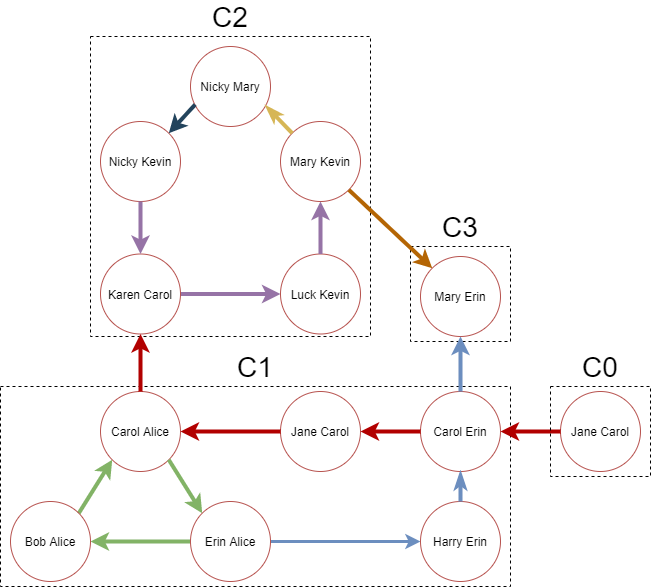
\includegraphics[width=\textwidth]{figures/uni-example.png}
    \caption{a tangle of four strongly connected components}
    \label{fig:uni-tangel}
\end{figure}

First, we prove that if every $c_i$ is concurrent, then there is a secure protocol. Since there is no cycle between $c_i$'s, there is a topological order between them. Consider the following algorithm.


\begin{algorithm}[H]
\label{alg:general_protocol}
\caption{Asynchronous Protocol}
\begin{algorithmic}
\State Let $\{c'_0, c'_1, .., c'_n\}$ is the topological order of $\mathcal{G}_s$ components.
\For{$i$ \textbf{from} $0$ \textbf{to} $n$}
\State Execute the synchronous protocol on $c'_i$
\EndFor
\end{algorithmic}
\end{algorithm}

Since each $c'_i$ is an cooperable tangle $T$, executing the synchronous protocol on each $c'_i$ is secure due to the result of theorem \ref{th:concurrency}. Hence, the entire execution process is secure.
% \begin{theorem}
% \label{th:opp-gen}
% Given a tangle $T$ and all of its strongly connected components in \genGraph graph $\{c_1, c_2, ..., c_n\}$, if there exists a $c_i$ which is not an executable concurrent tangle, then there is no tangle safe protocol for $T$.
% \end{theorem}
To prove the second direction of the theorem, we start by proving the following lemma:
\begin{lemma}
\label{lm:multiple-key-holder}
If there is a secure protocol for tangle $T$, then for each key, there is exactly one party who can own it.
\end{lemma}


We prove the lemma by contradiction. Assume in a concurrent tangle $T$ there are two parties $p_i$ and $p_j$ who are the key holder of the same lock. Then we prove that there is at least one party who may enter into the \underwater state. Given $\mathcal{G}_s=(V_g, E_g)$ assume $V_i \subset V$ and $V_j \subset V$ that for each $v \in V_i$, $p_i$ is the key holder and for each $v \in V_j$, $p_j$ is the key holder of the same stage. $\mathcal{G}_s$ is a strongly connected graph and for each $e \in E$ the same principal is overlapped between vertices $h(e)$ and $\tau(e)$, so the same lock is allowable on principals on both sides of $e$, hence $V_i \cap V_j$ can not be $\O$. Therefore, there is a swaption $s \in V_i \cap V_j$ that principals in $\beta(s)$ side and $\sigma(s)$ side are locked by different keys. Hence, if the key of one of these principals is revealed, its depositor will go \underwater.

% Therefore both parties in this swaption are threatened to be robbed and enter into underwater state. Because one of the $p_i$ may avoid to reveal its key while the other one reveals her key, then the principal which locked by the the revealed key will be transferred while other one will not. Thus the owner party of the transferred principal enters into the underwater state.

% that through the entire tangle there is no vertex $v$ that different locks are used for principal on vertices $v$ and $\mathcal{O}(v)$ in the same stage.
% swaption in which different locks are used for its outgoing black arcs. 
% Since 
% the outgoing arcs originating from the nodes of $p_1$ and $p_2$ have two different locks, whether there is two separately components on the \genGraph graph of the tangle or the same lock is used for all of the arcs in the tangle which is a contradiction. Thus there is a swaption which its ou\mathcal{G}_{t}oing black arcs are locked by different keys. Therefore The both parties in this swaption are threatened to be robbed and enter into underwater state. Because one of the $p_i$ may avoid to reveal its key while the other one reveals her key, then the arc which has the the revealed key will be triggered while other one will not. Thus the party corresponding to the triggered arc enters into underwater state.

% \ahC{Prove that source e $\mathcal{G}_{t}$ bayad keyone dastesh bashe.}

Now assume that there is a $c_i$ that is not cooperable tangle which means at least one of the following statements is true.

\begin{enumerate}
    \item $c_i$ is not \keyoneOk. Now, assume subgraph $\mathcal{G}_{t}=(V_t, E_t)$ of $\mathcal{G}_{p}$ for $c_i$ where $V_t=V$ and $E_t=\{e \in E | \rho(e) \neq t\}$. Then either $\mathcal{G}_{t}$ sources belong to different parties or the $\mathcal{G}_{p}$ has not any feedback edge set that satisfies the requirements of definition~\ref{def:pfok}. For the first case, there are at least two \keyone key holder parties in the graph. By the result of the lemma~\ref{lm:multiple-key-holder} there might be parties who go \underwater. In the second case, for each cycle $\mathcal{C}$ in $\mathcal{G}_{t}$ either for all edges $e \in \mathcal{C}$, $\rho(e)$ is $x$, thus the money transferring in $\mathcal{C}$ has to be the source of itself which is not acceptable, or for all edges $e \in \mathcal{C}$ that $\rho(e) \neq x$, $\tau(e)$ is not $p_{leader}$. If there is a protocol which executes $c_i$, to bypass this cycle, it must deviate from the principal deposition order imposed by edge $e \in \mathcal{C}$ that $\rho(e) \in \{i, t\}$. Hence the principal of the vertex $\tau(e)$ is forced to be deposited before the principal deposition of $h(e)$ while $\ell(\tau(e))$ is not $p_{leader}$. Then the party $\ell(h(e))$ can rob $\ell(\tau(e))$'s principal by cooperating with the graph key holders by early exposing all the keys.
    % there is at least one cycle $\mathcal{C}$ that 
    % has at least one insecure cycle. If there is more than one source in \keyoneGraph graph, then there are at least two parties in the graph who are the \keyone key holders. By the result of the lemma~\ref{lm:multiple-key-holder} it is a contradiction and there is a party who exits from the safe state. If there is an insecure cycle in the \keyoneGraphExtended graph, then there is a \textbf{Reversible} arc in this cycle. Since, if there is no such an arc in this cycle, then all of the arcs are black, hence the money which is transferring by these arcs has no source and comes from nowhere which is not acceptable. Therefore there must be at least one \textbf{Reversible} arc in this cycle. If there is a protocol which executes this tangle, to bypass the cycle, it must deviate from the principal deposition order imposed by one of the \textbf{Reversible} arcs in this cycle. Hence the party corresponding to the destination node of this arc is forced to deposit his principal before other party's deposition while he is none of the tangle key holders. Then the other party can robe his money by cooperating with the graph key holders by early exposing all the keys.
    
    % \ahC{We leave the case in which Bob deposits money from his own in multiple nodes} 
    
    % \ahC{alice and bob act as multiple nodes, it obviously fits in the scop of our proof}
    
    \item There is no party eligible to be the $p_{master}$ of $c_i$. 
   % \fatemeC{actually think pmaster is not defined on ci but anyway}:
    Then, if there is any protocol executing on $T$, then at least two locks are used for option funding stage. Hence, there is at least two key holders for the \Atwo key lock. Thus, there might be a party who goes \underwater.
    
\end{enumerate}

% Now we can define the swaptions universal theorem as a result of previously proved propositions:
% \begin{theorem}
% \label{th:universal}
% Given a tangle $T$, there is a safe protocol for executing $T$ if and only if every of $T$'s strongly connected components is an executable concurrent tangle.
% \end{theorem}

